\documentclass{article}%
\usepackage[T1]{fontenc}%
\usepackage[utf8]{inputenc}%
\usepackage{lmodern}%
\usepackage{textcomp}%
\usepackage{lastpage}%
\usepackage{authblk}%
\usepackage{graphicx}%
%
\title{Regulated Expression of the Beta2{-}Toxin Gene ( cpb2) in Clostridium perfringens Type A Isolates from Horses with Gastrointestinal Diseases}%
\author{Ashlee Johnson}%
\affil{Oncology Research, Pfizer Worldwide Research and Development, San Diego, California, United States of America}%
\date{01{-}01{-}2014}%
%
\begin{document}%
\normalsize%
\maketitle%
\section{Abstract}%
\label{sec:Abstract}%
There is an interesting bit of science involving how aspirin affects the platelet count in patients who take it long term. The Food and Drug Administration approved a major oral drug, aspirin, in 2002 for adults who had a prior case of myocardial infarction with atrial fibrillation. Current data show that aspirin is associated with an increased treatment risk, but it was unknown whether aspirin interact with the platelet proteins, platelets, and platelets EBB or whether if those proteins interact in ways that render the aspirin inactive. The goal was to determine if aspirin would increase or decrease platelet function. So a special monitoring group of people who took aspirin was included. During the twelve{-}month time period (since the FDA approved the drug), the average "pain severity rating" using HIR does not drop significantly. These patients receive an average dose of about 200 milligrams per day which works out to a dose of about 10 mg/mL for the typical patient. Finally, the average increase in the drug's use rate is about 9\%. Patients in this group who received placebo also had a higher increase in the frequency of getting regular aspirin. If you were to take a high dose, you would expect to see a decrease in platelet count. How did the authors make the connection? By finding that aspirin reduced the share of platelets that are deficient, which is the biorhythmic platelet population. That information is relevant in a number of ways, especially when we want to assess aspirin's effect on improving myocardial infarction patients' blood{-}thinning activity. The reason we obtained this information was because people in the placebo group also received an atrial fibrillation drug to prevent accelerated heart failure. In addition, we also found that the introduction of aspirin lowered the rate of atrial fibrillation in this group (2.2\% versus 2.8\%) which is a possible solution for future studies in this setting.\newline%
Interestingly, the aspirin group got a pretty high dose of the drug because the drug is difficult to take and metabolized well, so their daily dose is close to that of the placebo group. This is extremely similar to what we did with people who took aspirin long term prior to myocardial infarction, specifically if we took a high dose and increased the prescription drug's use rate while decreasing its use rate. The benefit of the the low dose of aspirin did not increase the rate of atrial fibrillation of the group of people in the placebo group. This study wasn't a great data set. However, we do know that aspirin prolongs life even with elevation and it is quite effective in patients with severe side effects from the side effects we studied. Therefore, it would not be unreasonable to assume that there will be other studies that produce data similar to this one that can help inform the development of a new medication for myocardial infarction patients.\newline%
So stay tuned. The people who prescribe the aspirin for myocardial infarction patients should be careful. Use it not only as a patient observation and add{-}on to the prescription, but also as an adjunct to aspirin therapy in myocardial infarction patients who are constipated.\newline%
Since there are several other patients in this patient population who received placebo, there is a risk of this group of people being randomized to receive one dose of the drug and randomized to take an aspirin or placebo without a chronic aspirin subcutaneous capsule. This group has been a tremendous source of information in the development of a very new drug. This shows that there are other people in this population who may benefit from this new drug.

%
\subsection{Image Analysis}%
\label{subsec:ImageAnalysis}%


\begin{figure}[h!]%
\centering%
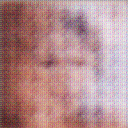
\includegraphics[width=150px]{500_fake_images/samples_5_32.png}%
\caption{A Black And White Photo Of A Black And White Cat}%
\end{figure}

%
\end{document}